\documentclass[a4paper,10pt]{article}
\usepackage[a4paper, left=3cm,right=2.5cm]{geometry}

\usepackage[spanish]{babel}
\selectlanguage{spanish}
\usepackage[utf8]{inputenc}
\usepackage[pdftex]{graphicx}

% Utilizado para recuadrar expresiones
\usepackage{amsmath}
% Recuadros con mayor separación
\setlength{\fboxsep}{6pt}

\def \anio {a\tilde{n}o}

\begin{document}

\paragraph{Ejercicio 1} A continuación se presenta la red, con el camino crítico resaltado en trazo grueso; esta comprende las actividades B, C, D, E y J. La duración del proyecto es de 23 semanas.

    \begin{center}
	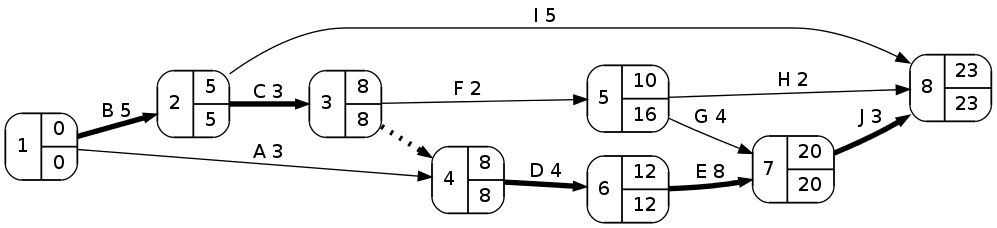
\includegraphics[scale=0.55,keepaspectratio=true]{img/ej1-red.png} 
	\end{center}
  
\paragraph{Ejercicio 3}
  Para encontrar el camino crítico, se obtiene el grafo de tareas representado por la matriz de precedencia y, sobre el mismo, se ejecuta el algoritmo de búsqueda de camino crítico.

  \begin{center}
    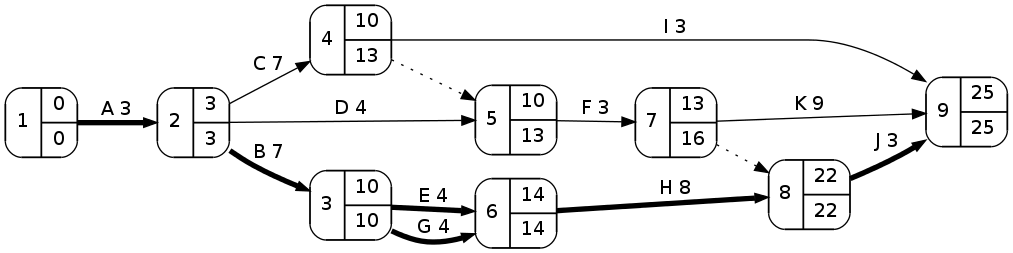
\includegraphics[scale=0.4,keepaspectratio=true]{img/ej3-0.png} 
  \end{center}

  El este gráfico puede verse el proyecto inicial, con los caminos críticos resaltados en trazo más grueso y las tareas ficticias en líneas punteadas.

  Los caminos críticos son: A-B-E-H-J y A-B-G-H-J.

  La duración del proyecto es de 25 semanas. Y, su costo, es de \$$14600$ (se obtiene sumando el costo de cada tarea, consistente en el producto de su duración por el costo semanal de la misma).

  \subparagraph{Reducción de la duración del proyecto}

  Para poder decidir el orden en que se reducirán las tareas, se calcula el costo de reducción semanal de cada una. Éste se obtiene como el cociente entre el costo de reducción total ($\Delta \$$ o costo crash menos costo) y su máxima reducción posible ($\Delta d$ o diferencia entre tiempo normal y tiempo mínimo).

   \begin{center}
   \begin{tabular}{|| c | c | c | c ||}
   \hline 
      Tarea & $\Delta d$ & $\Delta \$$ & $\Delta \$ / \Delta d$ \\ \hline \hline
      A & 1 & 100 & 100 \\ \hline
      B & 1 & 140 & 140 \\ \hline 
      C & 2 & 400 & 200 \\ \hline
      D & 2 & 500 & 250 \\ \hline
      E & 2 & 400 & 200 \\ \hline
      F & 2 & 600 & 300 \\ \hline
      G & 3 & 900 & 300 \\ \hline
      H & 0 &  -  & -   \\ \hline
      I & 1 &1000 & 1000\\ \hline
      J & 0 &  -  & -   \\ \hline
      K & 3 & 300 & 100 \\ \hline
   \end{tabular}
   \end{center}

   Puede verse en la tabla que la tarea crítica con menor costo de reducción semanal es A. Sin embargo ésta puede reducirse a lo sumo en una semana. Por lo tanto, si conviene, deberá luego reducirse otra tarea.

  \subparagraph {Reducción en una semana de la tarea A}
  \begin{center}
    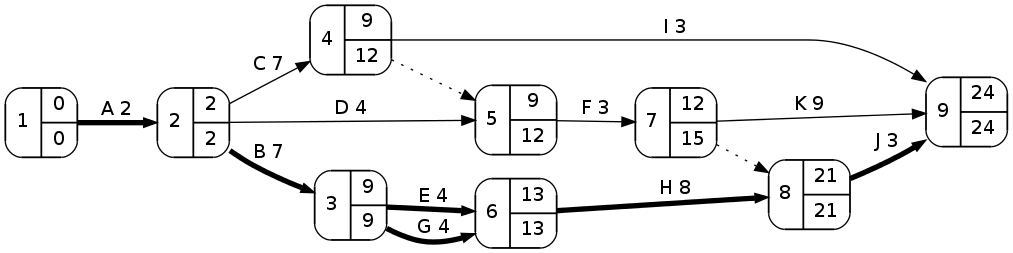
\includegraphics[scale=0.4,keepaspectratio=true]{img/ej3-1.png} 
  \end{center}

  Al haber reducido una tarea crítica en una semana, la nueva duración del proyecto es de 24 semanas. Y su nuevo costo, dado el beneficio otorgado por esta reducció, es de $\$14600 - \$150 + \$100 = \$14550$. Por lo tanto, conviene reducir el proyecto en una semana.


  Ahora, la tarea crítica con menor costo de reducción semanal es B.

  \subparagraph {Reducción en una semana de la tarea B}
  \begin{center}
    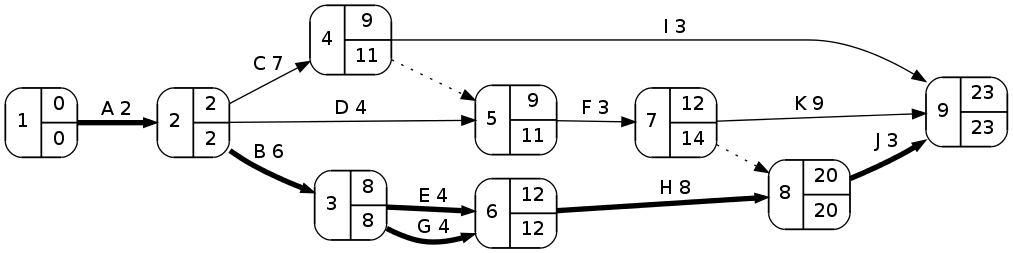
\includegraphics[scale=0.4,keepaspectratio=true]{img/ej3-2.png} 
  \end{center}

  Nuevamente bajó la duracción del proyecto, a un total de 23 semanas. Y su costo ahora es de $\$14550 - \$150 + \$140 = \$14540$. Entonces conviene aceptar la reducción de 25 a 23 semanas.

  \subparagraph {Reducción de la tercer semana}
  Ahora, la única reducción posible en tareas que formen parte de un camino crítico es en E y G. Dado que ambas no forman parte del mismo camino, deben reducirse en simultáneo.

  El costo de reducir en una semana E es de $\$200$, y el de G es de $\$300$, por lo que no conviene si el beneficio percibido es de $\$150$ en total ya que el nuevo costo llegaría a ser de $\$14540 + \$200 + \$300 - \$150 = \$14890$, siendo mayor que el original del proyecto.



\paragraph{Ejercicio 5}

Para comenzar el ejercicio, se comienza planteando el gr\'afico de la red planteada en el enunciado y se marca con l\'inea m\'as gruesa y roja el camino cr\'itico en cuesti\'on.

  \begin{center}
    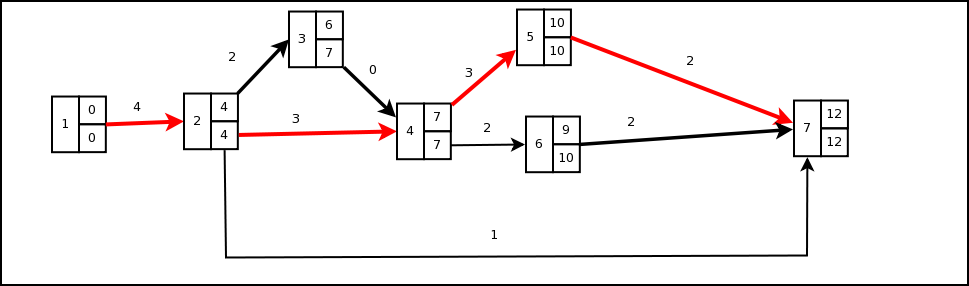
\includegraphics[scale=0.4,keepaspectratio=true]{img/ej5-red.png} 
  \end{center}

\subparagraph {5.a}
Para lograr reducir la duraci\'on del proyecto en 2 d\'ias, tal cual solicita el enunciado, se plantear\'a el m\'etodo de acortamiento de proyectos. //
Dicho m\'etodo plantea la obtenci\'on del tiempo en el que puede reducirse una tarea ( obteniendose como la diferencia entre la duraci\'on y el tiempo m\'inimo de ejecuci\'on para cada tarea) y 
considerando el costo para reducir en un d\'ia dicha tarea. Se plantea la siguiente tabla:

   \begin{center}
   \begin{tabular}{|| c | c | c | c ||}
   \hline 
      Tarea & $\Delta d$ & Inc. de costo por reducci\'on en un d\'ia \\ \hline \hline
      1-2 & 1 & 600  \\ \hline
      2-3 & 1 & 500  \\ \hline 
      2-4 & 2 & 1000  \\ \hline
      2-7 & 0 & - \\ \hline
      3-4 & 0 & - \\ \hline
      4-5 & 1 & 700 \\ \hline
      4-6 & 1 & 200 \\ \hline
      5-7 & 1 & 400    \\ \hline
      6-7 & 1 & 400\\ \hline
   \end{tabular}
   \end{center}

A continuaci\'on se calcula el presupuesto del proyecto como la suma de los costos de cada una de las tareas, entonces:

$$ Presupuesto = 1400 + 1500 + 1600 + 600 + 1300 + 800 + 300 + 6000 = \$13500$$

Seg\'un se desprende del camino cr\'itico planteado en el gr\'afico anterior, comprendido por las tareas: $1-2-4-5-7$ la duraci\'on total del proyecto es de 12 d\'ias.
\\
De acuerdo con la metodolog\'ia de acortamiento de proyectos, se comienza por reducir en un d\'ia el proyecto en cuesti\'on. Para ello, se analiza de las tareas que conforman dicho camino cr\'itico 
y poseen un $\Delta d$ mayor que 0, aquella que posee un Inc. de costo por reducci\'on en un d\'ia menor.\\

La tarea seleccionada para reducir es la 5-7, con lo cual, la tabla anterior quedar\'ia:


   \begin{center}
   \begin{tabular}{|| c | c | c | c ||}
   \hline 
      Tarea & $\Delta d$ & Inc. de costo por reducci\'on en un d\'ia \\ \hline \hline
      1-2 & 1 & 600  \\ \hline
      2-3 & 1 & 500  \\ \hline 
      2-4 & 2 & 1000  \\ \hline
      2-7 & 0 & - \\ \hline
      3-4 & 0 & - \\ \hline
      4-5 & 1 & 700 \\ \hline
      4-6 & 1 & 200 \\ \hline
      5-7 & 0 & 400    \\ \hline
      6-7 & 1 & 400\\ \hline
   \end{tabular}
   \end{center}

A continuaci\'on se muestra la nueva red, luego de calcular las fechas tempranas y tard\'ias considerando la reducci\'on realizada:

  \begin{center}
    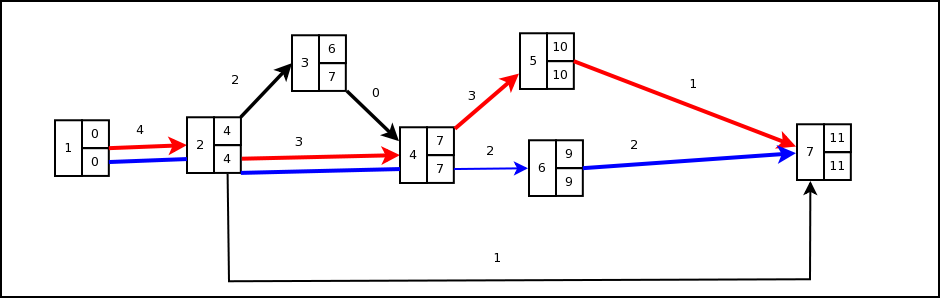
\includegraphics[scale=0.4,keepaspectratio=true]{img/ej5-1red.png} 
  \end{center}

El nuevo presupuesto del proyecto se calcula como:

$$ Presupuesto = \$13500 + \$400 = \$13900 $$

Del gr\'afico se desprende que la nueva duraci\'on del proyecto es de 11 d\'ias y surge, adem\'as del ya existente, un nuevo camino cr\'itico. Este nuevo camino est\'a
comprendido por $1-2-4-6-7$.

Analizando ambos caminos cr\'iticos en conjunto, se desprende que la tabla sobre la que debe analizarse la posible reducci\'on para disminuir en un d\'ia mas la duraci\'on total del proyecto es la siguiente:

   \begin{center}
   \begin{tabular}{|| c | c | c | c ||}
   \hline 
      Tarea & $\Delta d$ & Inc. de costo por reducci\'on en un d\'ia \\ \hline \hline
      1-2 & 1 & 600  \\ \hline
      2-4 & 2 & 1000  \\ \hline
   \end{tabular}
   \end{center}

Elijo reducir la tarea 1-2 dado que es la que posee un menor Inc de reducci\'on en un d\'ia, la tabla en cuesti\'on es la siguiente:

   \begin{center}
   \begin{tabular}{|| c | c | c | c ||}
   \hline 
      Tarea & $\Delta d$ & Inc. de costo por reducci\'on en un d\'ia \\ \hline \hline
      1-2 & 0 & 600  \\ \hline
      2-4 & 2 & 1000  \\ \hline
   \end{tabular}
   \end{center}


Realizando esta modificaci\'on en la red anterior y recalculando la nueva fecha temprana y tard\'ia para cada una de las tareas se obtiene la siguiente red:

  \begin{center}
    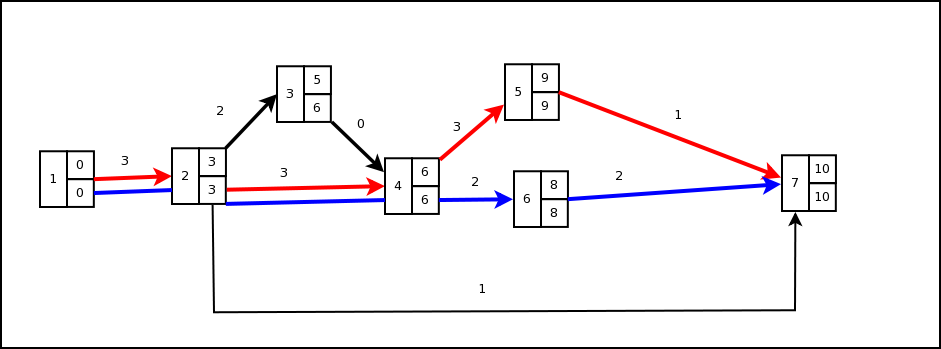
\includegraphics[scale=0.4,keepaspectratio=true]{img/ej5-2red.png} 
  \end{center}

El nuevo presupuesto del proyecto se calcula como:

$$ Presupuesto = \$13900 + \$600 = \$14500 $$

Del gr\'afico se desprende que la nueva duraci\'on del proyecto es de 10 d\'ias.\\

Por lo tanto, se puede concluir que para que el proyecto finalice 2 d\'ias antes es necesario un presupuesto de $\$14500$

\subparagraph {5.b}

En el ejercicio se propone calcular la cantidad de d\'ias en la que conviene finalizar el proyecto de forma tal de minimizar los costos considerando que a partir del d\'ia 11 se cobrar\'a un inter\'es
de \$100 por d\'ia.\\
Utilizando lo calculado en el ejercicio anterior, se observa que, para finalizar el proyecto en 11 d\'ias es necesario incrementar el costo en \$400 y por finalizarlo en 10 d\'ias (momento a partir del cual ya no se 
cobra inter\'es), es necesario incrementar el costo en \$1000. \\

Por lo tanto, considerando que se cobran \$100 por el d\'ia 11 y \$100 por el d\'ia 12 como inter\'es, es decir se incrementar\'a en \$200 el total del proyecto, se puede deducir que 
es conveniente dejar que el proyecto finalice en los 12 d\'ias en los cuales fue planificado dado que es necesario un presupuesto total de \$13700, considerando el inter\'es. Este costo es 
\$200 menor que el necesario para finalizarlo en 11 d\'ias como fue calculado en la parte a del presente ejercicio.





\end{document}
